\section{Aufbau}
\label{sec:aufbau}

Der Aufbau dieses Versuchs wird im nachfolgenden Abschnitt genauer erklärt, da dessen Funktionsweise nötig für die korrekte Durchführung ist.
Das komplette Schaltbild ist in \autoref{fig:szintillator} dargestellt.
\begin{figure}
    \centering
    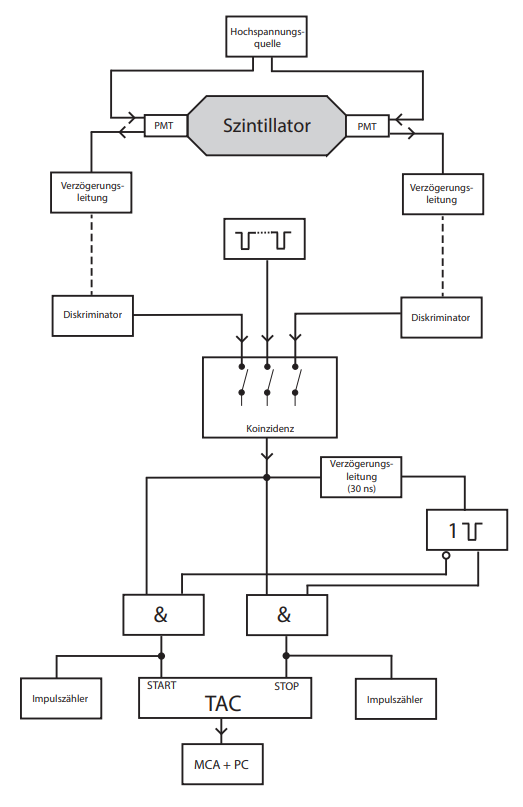
\includegraphics[width=0.8\textwidth]{content/images/szintillator.png}
    \caption{Skizze der verwendeten Schaltung. Im oberen Teil der Schaltung werden Signale detektiert und im unteren Teil die Zeit zwischen den Signalen gemessen. \cite{V01}}
    \label{fig:szintillator}
\end{figure}
Die eigentliche Detektion der Myonen findet mit einem Szintillator statt.
Dieser wird aufgrund der eintreffenden geladenen Teilchen ionisiert und emittiert Licht.
Die angeschlossenen Photomultiplier (PMT) werden über einen Hochfrequenzgenerator betrieben und verstärken die eintreffenden Photonen zu einem elektrischen Signal.
\\
Das entstandene Signal wird beidseitig aus dem Szintillator jeweils in eine Verzögerungsleitung geschickt.
Eine Verzögerungsleitung besitzt eine variable Leitungslänge, womit das elektrische Signal zeitlich verzögert werden kann.
Anschließend gelangen die Signale in einen Diskriminator.
Sollte das Signal eine festgelegte Signalstärke übersteigen, wird es in einn Rechtecksignal umgewandelt, dessen Signallänge eingestellt werden kann.
Die Nutzung von zwei Diskriminatoren verhindert, dass spontan ausgelöste Signale der Photomultiplier als Myon gezählt werden.
Wird im Szintillator also ein Myon detektiert, sollten zwei Signale aus den beiden Diskriminatoren an die Koinzidenz übermittelt werden.
Nur wenn innerhalb einer eingestellten Koinzidenzzeit zwei Signale die Koinzidenz erreichen, gibt sie ein Signal in den zweiten Teil der Schaltung weiter.
\\
Das Signal aus der Koinzidenz wird hier aufgeteilt.
Einerseits gelangt das Signal zu einem AND-Gatter, das als Startpunkt der Zerfallszeit dient.
Ein AND-Gatter benötigt jedoch zwei aktivierte Eingänge um ein Signal weiterzugeben.
Der zweite Eingang ist mit einem Monoflop verbunden, welcher in seinem Grundzustand über normale Ausgänge kein Signal ausgibt und über invertierte Ausänge ein Signal.
Das Start AND-Gatter ist mit einem invertierten Ausgang verbunden.
Es wird also aktiviert, sobald ein Signal der Koinzidenz es erreicht.
Dadurch wird ein Impulszähler aktiviert, welcher die Anzahl aller Start-Impule mitzählt.
Außerdem wird der Start-Eingag des TAC (\textit{Time amplitude converter}) aktiviert.
Dieser misst die Zeitdifferenz zwischen Start- und Stoppsignal und wandelt diese in eine Amplitude um.
\\
Das Stoppsignal kann erst gemessen werden, nachdem sich die Schaltung in einen neuen Zustand begibt.
Denn das ursprüngliche Signal aus der Koinzidenz wird außerdem über eine Verzögerungsleitung um etwa ZEIT NACHSCHAUEN verzögert und dann an den Monoflop übertragen.
Daraufhin begibt sich der Monoflop in einen angeregten Zustand. 
Alle Ausgänge ändern somit ihr Ausgangssignal.
Das inverse Signal, welches an das Start AND-Gatter geleitet wird, ist jetzt deaktivert und verhindert so weitere Startmessungen.
Allerdings aktiviert ein nicht invertierter Ausgang nun den Stopp AND-Gatter.
Dieser angeregte Zustand wird für eine Suchzeit $T_\text{s}$ beibehalten. 
In dieser Zeit wird auf ein Signal der Elektronen, die aus dem Myonzerfall entstanden sind, gewartet.
Dieses Zerfallssignal durchläuft den ersten Teil der Schaltung und gibt über die Koinzidenz ein Signal an das Stopp AND-Gatter.
Dort sind nun beide Eingänge aktiviert und analog zum Start AND-Gatter wird der Impuls gezählt und an den TAC weitergegeben.
Dieser beendet seine Messung und übergibt die Amplitude an den Vielkanalanalysator.
Sollte innerhalb der Suchzeit kein weiteres Signal eintreffen, begibt sich der Monoflop wieder in den Grundzustand und eine neue Startmessung kann beginnen.
Der Vielkanalanalysator erhält alle im Experiment gemessenen Zerfallszeiten und trägt sie in einem Histogramm auf.
Es wird dort gezählt wie oft welche Zerfallszeit gemessen wurde und sollte eine Exponentialverteilung darstellen, die dem Zerfallsgesetzt entspricht.